\documentclass[pdftex]{beamer}
\usetheme[author,date,title]{lines}
\usecolortheme{aptero}
 
\usepackage{beamerthemelines}
\usepackage{hyperref}
\usepackage{multimedia}
\usepackage{wasysym}

%\usepackage{ngerman}			% language set to new-german
\usepackage[english]{babel}		% language set to new-german
\usepackage[utf8]{inputenc} 	% coding of german special characters

\usepackage{graphicx}  % \includegraphics[options]{file.eps}
\usepackage{tikz}
\usepackage{tikz}
\graphicspath{{images/}}
%\usepackage{array}
\usepackage{setspace}
\usepackage{scalerel}
\usepackage{color}
\usepackage{colortbl}
\usepackage{eqlist}
\usepackage{pgfgantt}
\usepackage{wallpaper}
\usepackage[percent]{overpic}

\newcommand{\paper}[1]{\footnotesize{\textit{#1}}\normalsize{}}

\setlength{\unitlength}{0.01\paperwidth}


% Setup of listings
\usepackage{listings}
\lstset{language=bash,
  backgroundcolor=\color{black},
  tabsize=3, aboveskip=0.5cm,
  belowskip=0.5cm, breaklines=true,captionpos = b, numbers=left,
  firstnumber=1, numberstyle=\tiny, xleftmargin=20pt, frame=single,
  framerule=0.25pt, showstringspaces=false, stringstyle=\color{white}}

\definecolor{lstbg}{rgb}{0.9,0.9,0.9}

\graphicspath{{../../../images/}}

\title[NIX - Neo workshop]{INCF virtual training weeks 2021 \\ -- NIX Neo workshop -- }
\author[]{Michael Denker, Jan Grewe, Julia Sprenger, \& Michael Sonntag}
\institute[G-Node]{German Neuroinformatics Node}
\date[30.08 - 01.09]{August 30, 2021 -- September 01, 2021}
%\logofootright{
\includegraphics[height=3.5ex]{resources/G-Node-logo.png}}
%\logofootleft{
\includegraphics[height=5ex]{resources/nix_logo.png}\hfill}%
%  \includegraphics[height=6ex]{BCCN_Tuebingen_Logo-long}\hfill%
%  \includegraphics[height=5ex]{CIN-E}}
\titlelogo{
\includegraphics[height=10ex]{resources/nix_logo.png}\hfill

\includegraphics[height=10ex]{resources/G-Node-logo.png}}
%  \includegraphics[height=5ex]{CIN-E}}

%%%%%%%%%%%%%%%%%%%%%%%%%%%%%%%%%%%%%%%%%%%%%%%%%%%%%%%%%%%%%%%%%%%%%%%%%%%%
\begin{document}
%%%%%%%%%%%%%%%%%%%%%%%%%%%%%%%%%%%%%%%%%%%%%%%%%%%%%%%%%%%%%%%%%%%%%%%%%%%%

\begin{frame}[plain]
  \titlepage{}
\end{frame}


\begin{frame}{Reproducibility crises}
    \begin{center}
        \only<1> {
        \begin{overpic}[width=0.75\textwidth]{resources/rung_brazma_2013.png}
            \put (-20, 15) {
            \begin{quotation}[Rung \& Brazma, 2012]
            The authors replicated two studies ‘in principle’ and six ‘partially’, whereas ten were not reproduced. [...]The main reason for the lack of reproducibility was the unavailability of all relevant data or metadata.
            \end{quotation}
            }
        \end{overpic}
        } \only<2> {
        \begin{overpic}[width=0.75\textwidth]{resources/hines_etal_2014.png}
            \put (-20, 20) {
            \begin{quotation}[Hines et al., 2014]
            ... our two laboratories quite reproducibly were unable to replicate each other’s fluorescence-activated cell sorting (FACS) profiles of primary breast cells.
            \end{quotation}
            }
        \end{overpic}
        }
    \end{center}
\end{frame}

\begin{frame}{Reproducibility crisis}
    "Challenges in irreproducible research", Nature special, 06.07.2018, ISSN 1476-4687 \url{https://www.nature.com/collections/prbfkwmwvz}
    \vspace{1cm}
    \begin{quotation}
        "More than 70\% of researchers have tried and failed to reproduce another scientist's experiments, and more than half have failed to reproduce their own experiments. Those are some of the telling figures that emerged from Nature's survey of 1,576 researchers who took a brief online questionnaire on reproducibility in research."
    \end{quotation}
\end{frame}

\begin{frame}{Reproducibility crisis}
    What factors contribute to irreproducible research?
    \begin{itemize}
        \item <1-> Selective reporting
        \item <1-> Pressure to publish
        \item <1-> Low statistical power or poor analysis
        \item <1-> Not replicated enough in original lab
        \item <1-> Insufficient oversight/mentoring
        \item <1-> Methods \& code unavailable
        \item <1-> Poor experimental design
        \item <1-| alert@2> Raw data not available from original lab
        \item <1-> Fraud
        \item <1-> Insufficient peer review
        \item <1-> Problems with reproduction efforts
        \item <1-> Technical expertise required for reproduction
        \item <1-> Variability of standard reagents
        \item <1-> Bad luck
        \item <1-| alert@2> Insufficient metadata
    \end{itemize}
\end{frame}

\begin{frame}{Reproducibility crisis also in the Neurosciences}
    \large{There is a lack of standardization} \vspace{1ex}
    \begin{itemize}
        \item <1-> Earlier (roughly 2007/2008) this was also identified as one problem in neuroscience. \vspace{1ex}
        \item <2-> We need standards and tools to help doing good neuroscience.  \vspace{1ex}
        \item <3-> The INCF task force on \textbf{Standardization in electrophysiology} was the starting point of the NIX project.
    \end{itemize}
\end{frame}

\begin{frame}{Reproducibility crisis also in the Neurosciences}
    \begin{center}
        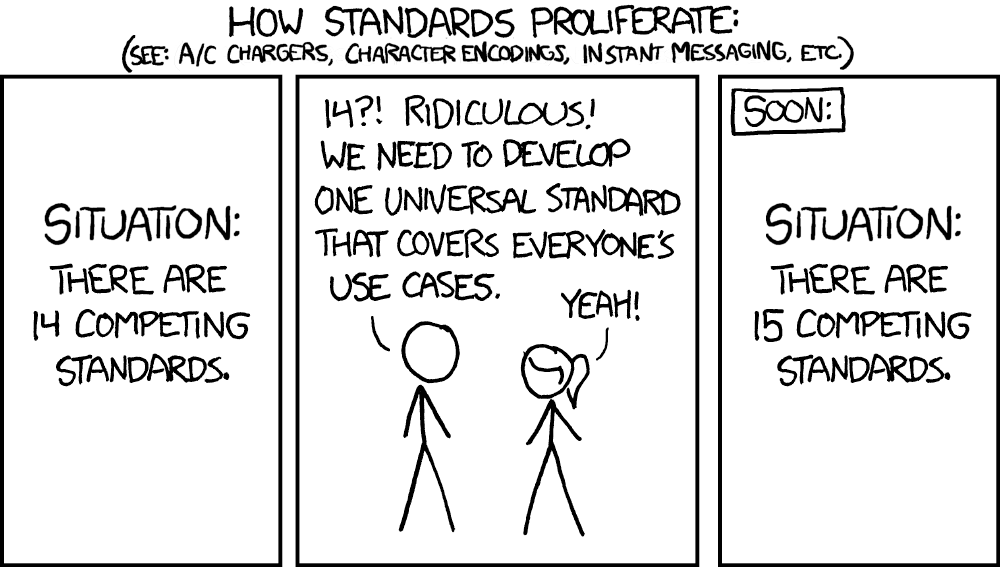
\includegraphics[width=0.75\columnwidth]{resources/standards}\rotatebox{90}{\url{https://xkcd.com/927}}
    \end{center}
    \pause
    ... but at least some of these are \textbf{open-source}!
\end{frame}


\begin{frame}{NIX}
    \begin{center}
        
\includegraphics[width=0.35\columnwidth]{resources/nix_logo}\\
        \vspace{2ex}
        \textbf{N}euroscience \textbf{I}nformation E\textbf{x}change\\
        \vspace{2ex}
        Originates from the neuroscience ...\\but is not limited to it.
    \end{center}
\end{frame}


\begin{frame}{NIX concept}
    NIX aims at:
    \begin{enumerate}
        \item One data model for storing data and metadata within the same container.
        \item Flexible enough to support a high variety of data types.
        \item Store n-dimensional data.
        \item Allow in-depth annotations.
        \item Data entities are self describing.
        \item Support standardization in data and metadata storing.\vspace{2ex}
        \item Of course, open source.
    \end{enumerate}
\end{frame}


\begin{frame}{NIX Data Model}
    \begin{center}
        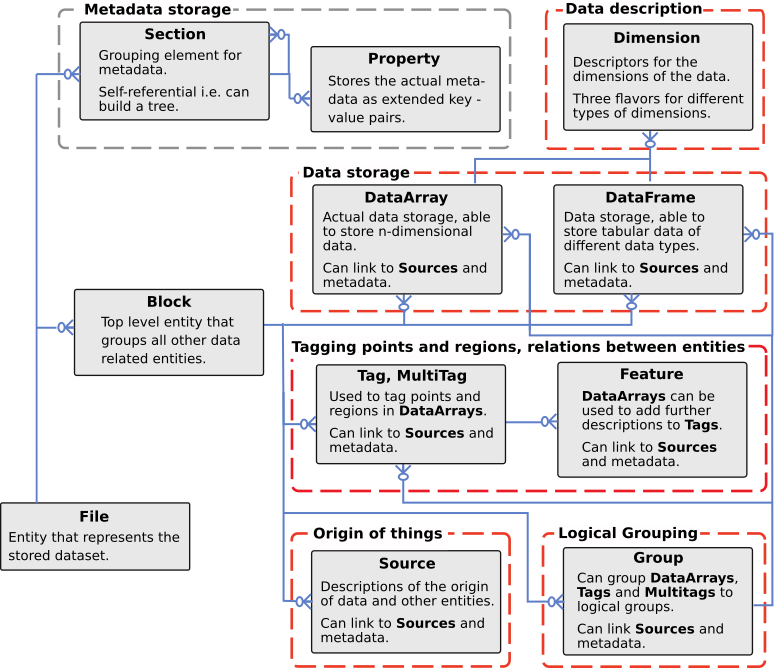
\includegraphics[width=0.7\columnwidth]{../day_1/resources/data_model_overview}
    \end{center}
\end{frame}


\begin{frame}{NIX Data Model}
    \begin{center}
        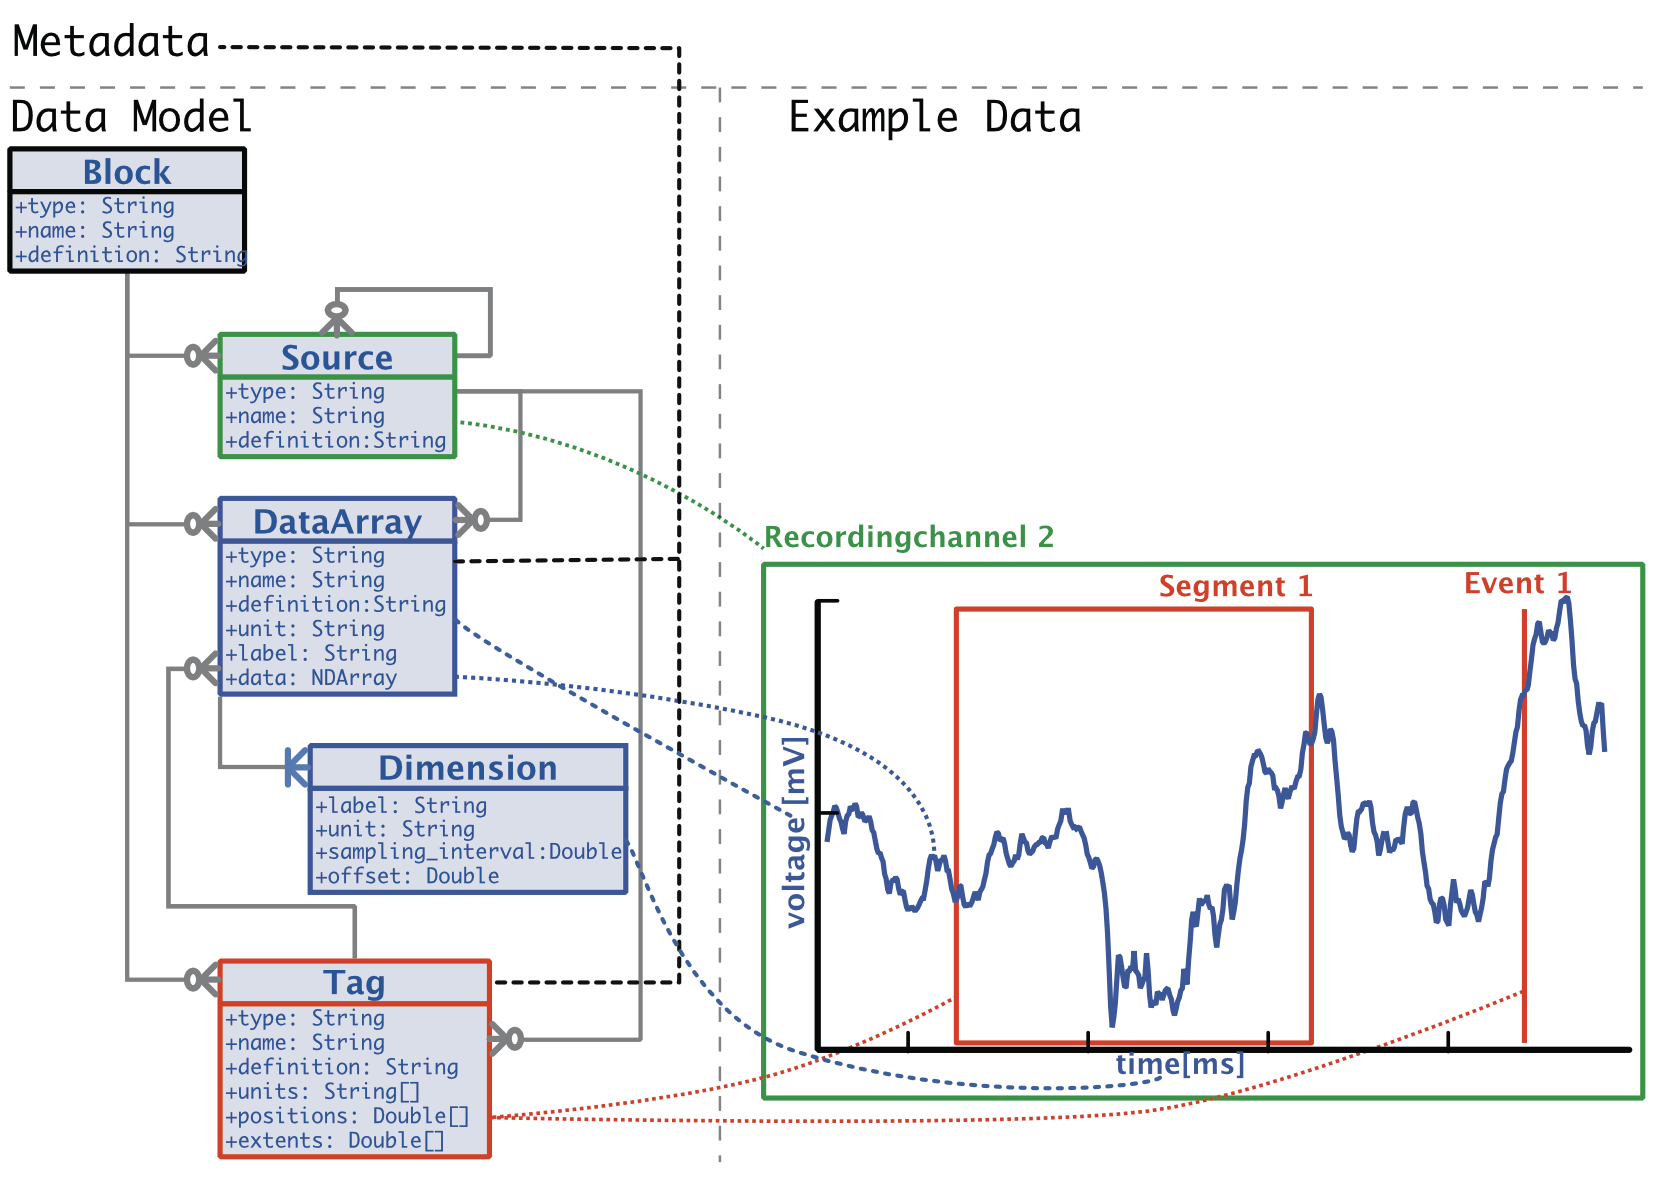
\includegraphics[width=0.75\columnwidth]{../day_1/resources/example_signal}
    \end{center}
\end{frame}


\begin{frame}{NIX Data Model}
    \begin{itemize}
        \item The NIX data model is not a file format.
        \vspace{1ex}
        \item It can be implemented in many backends.
        \vspace{1ex}
        \item So far, we use the HDF5 file format as storage backend.
    \end{itemize}
\end{frame}


\begin{frame}{NIX Implementations}
    \begin{center}
        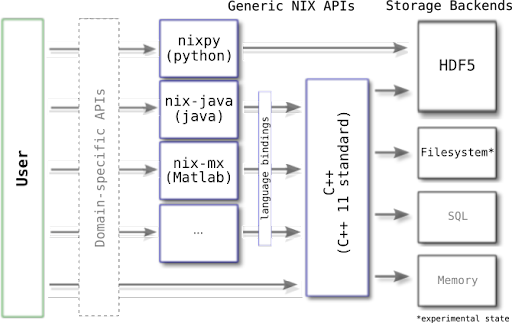
\includegraphics[width=0.85\columnwidth]{resources/nix_apis}
    \end{center}
\end{frame}


\begin{frame}{Generic APIs}
    \begin{columns}
        \begin{column}{6cm}
            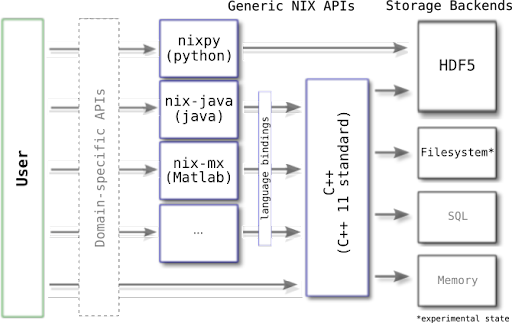
\includegraphics[width=\columnwidth]{resources/nix_apis}
        \end{column}
        \begin{column}{6.5cm}
            \begin{itemize}
                \item There are two native APIs: nixpy (python) and nixio (C++) and two that use language bindings to write NIX files to HDF5 files.
                \vspace{1ex}
                \item In principle, we can support several different backends. 
            \end{itemize}
        \end{column}
    \end{columns}
\end{frame}


\begin{frame}{Domain specific APIs}
    \begin{columns}
        \begin{column}{6cm}
            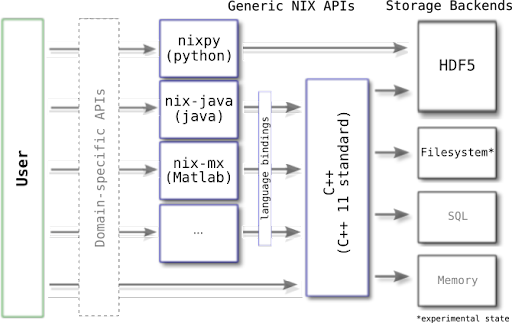
\includegraphics[width=\columnwidth]{resources/nix_apis}
        \end{column}
        \begin{column}{6.5cm}
            \begin{itemize}
                \item Domain specific APIs use the generic ones to ease access to data from one domain, e.g. Electrophysiology.
                \vspace{1ex}
                \item They provide a way to adapt and standardize storing data.
                \item This does not hinder to read the data with the generic libraries.
            \end{itemize}
        \end{column}
    \end{columns}
    \vspace{2ex}
    $\Rightarrow$ Neo-nixio stores Neo electrophysiology data using NIX as storage backend.\\
    \vspace{1ex}
    $\Rightarrow$ Storing to NIX can be embedded into the recording software \url{http://relacs.sourceforge.net}.
\end{frame}

\begin{frame}{Reproducibility crisis also in the Neurosciences}
    \begin{center}
        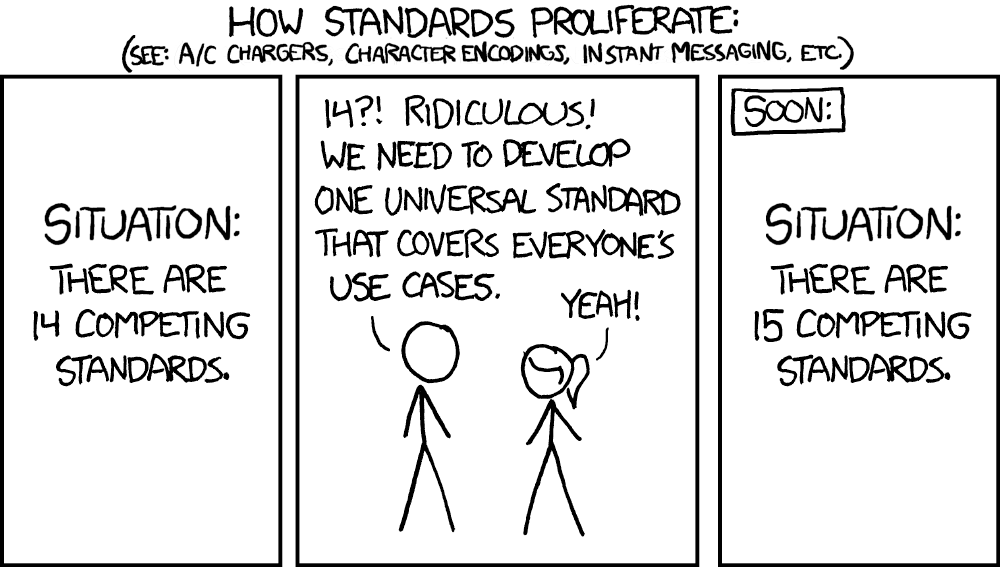
\includegraphics[width=0.75\columnwidth]{resources/standards}\rotatebox{90}{\url{https://xkcd.com/927}}\\
        \vspace{1ex}
        \textit{...and the other 40+ ephys data standards?}
    \end{center}
\end{frame}


\begin{frame}{Neo}
    \begin{columns}
        \begin{column}{6.5cm}
            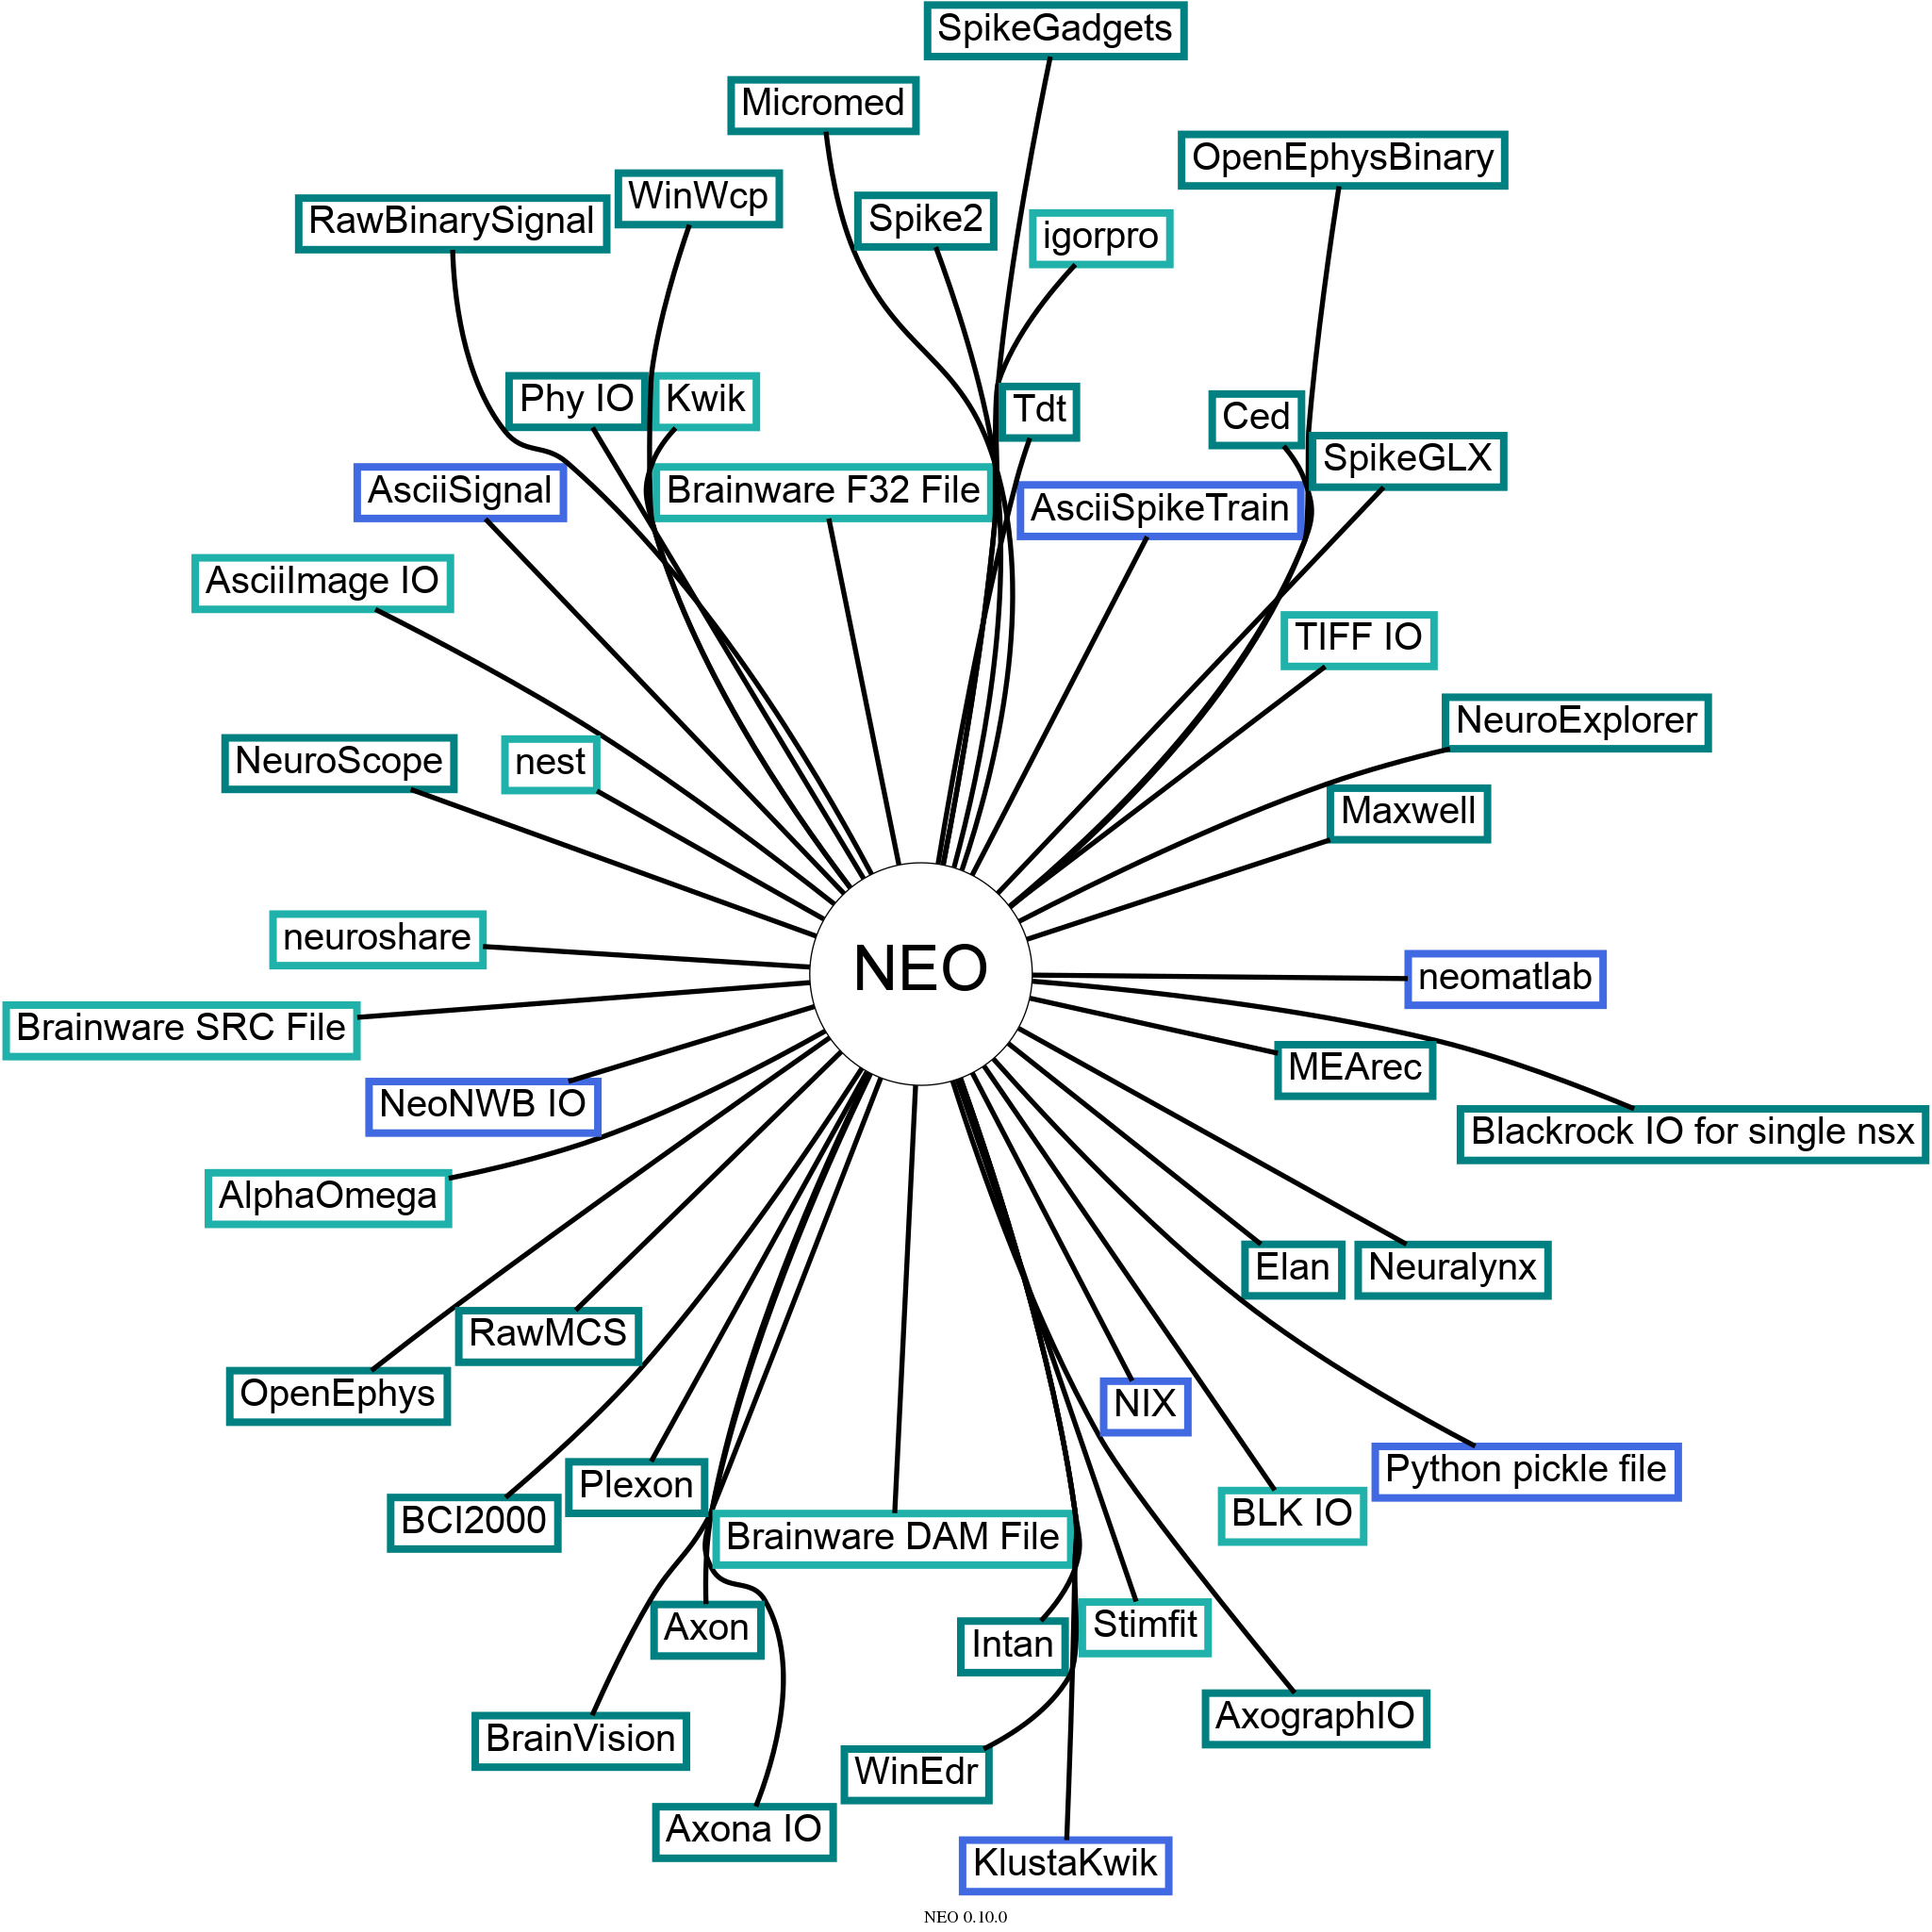
\includegraphics[height=.8\textheight]{resources/neo_IODiagram.png}
        \end{column}
        \begin{column}{5.5cm}
        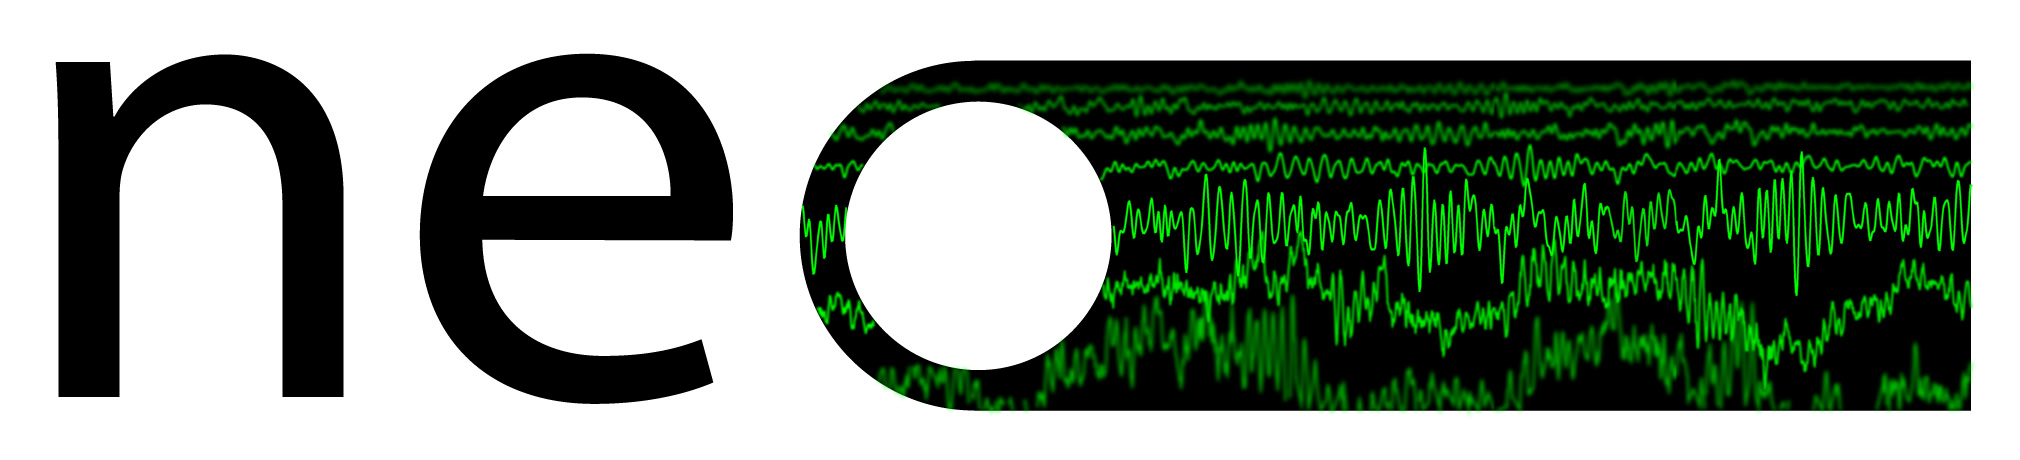
\includegraphics[width=4cm]{resources/neo_logo_transparent.png}
            \begin{itemize}
                \item interfaces to 40+ ephys proprietary \& open formats in various versions
                \vspace{1ex}
                \item provides a standardized ephys data \textbf{representation}, it is not a file format.
                \item reads all formats, but provides writing capability only for selected open formats.
            \end{itemize}
        \end{column}
    \end{columns}
\end{frame}


\begin{frame}{Neo}
    A basis for
    \begin{itemize}
        \item format conversion
        \item custom data analysis
        \item diverse tools dealing with ephys data
    \end{itemize}
    \vspace{1ex}
    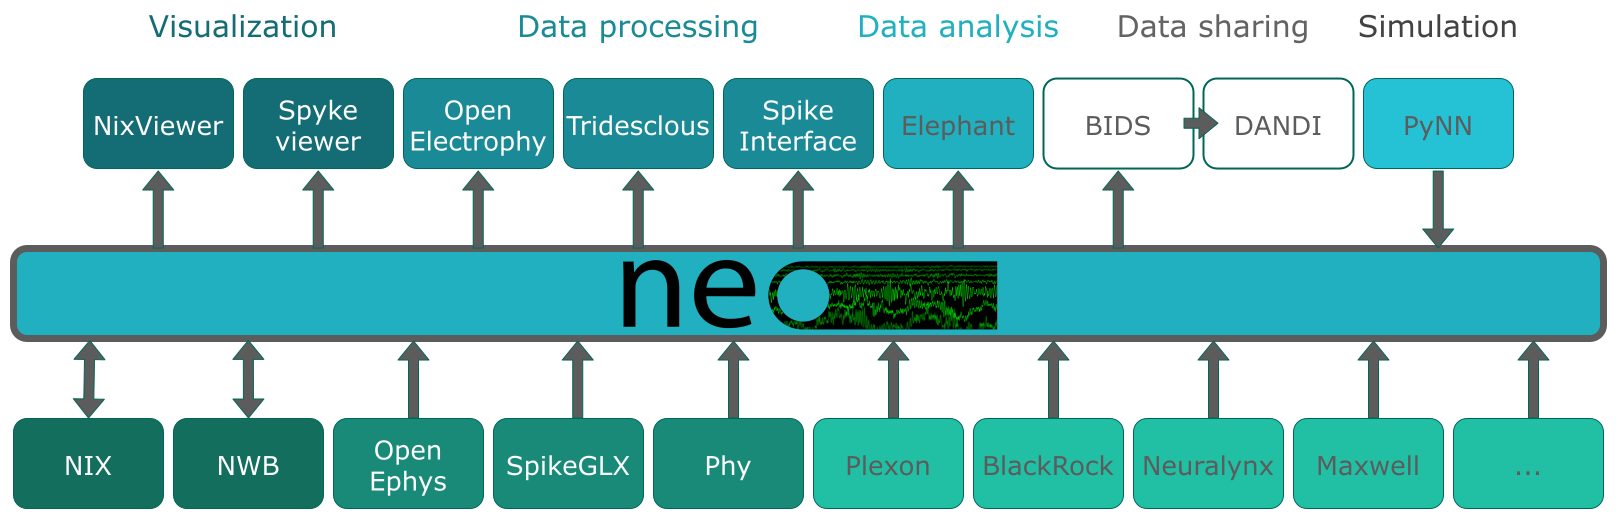
\includegraphics[width=\textwidth]{resources/neo_as_interface.png}
\end{frame}


\begin{frame}{Elephant}
    \begin{center}
    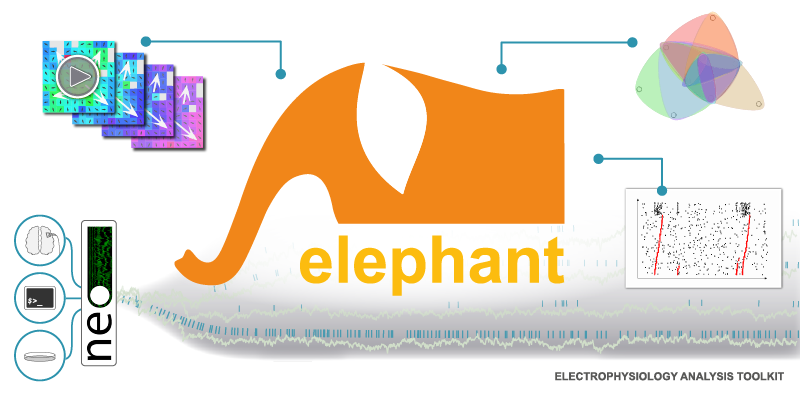
\includegraphics[width=.7\textwidth]{resources/elephant_teaser.png}\\
    \ \\
    Electrophysiology Analysis Toolkit
    \begin{itemize}
        \item analysis of brain activity (spike trains, local field potentials,\dots)
        \item builds on the Neo framework (input, output)
        \item focus on population measures from experiment and simulation
    \end{itemize}
    \end{center}
\end{frame}


\begin{frame}{Viziphant}
    \begin{columns}
        \begin{column}{6cm}
            
\includegraphics[width=\textwidth]{resources/viziphant_logo_sidebar.png}
        \end{column}
        \begin{column}{6cm}
            Quick visualizations
            \begin{itemize}
                \item of Neo representations of electrophysiology data
                \item of Elephant analysis results
            \end{itemize}
        \end{column}
    \end{columns}
\end{frame}




\begin{frame}{NIX-Neo Workshop}
    In this workshop we will ...
    \begin{itemize}
        \item introduce the ideas and concepts of the NIX data model.
        \item show how various data types can be represented with it.
        \item show how to use and find data in NIX files.
        \item become familiar with the Neo representation of electrophysiology data.
        \item learn how to used Elephant and Viziphant for data analysis and visualizations.
        \item use a lot of hands-on exercises.
    \end{itemize}
\end{frame}


\begin{frame}{NIX-Neo Workshop}
    \begin{columns}[t]
        \begin{column}{4cm}
            \textbf{Day 1:} NIX Basics\vspace{1ex}
            \begin{itemize}
                \item Introduction
                \item File \& data handling
                \item Tagging
                \item Annotations
            \end{itemize}
        \end{column}
        \begin{column}{4cm}
            \textbf{Day 2:} Deeper dive\vspace{1ex}
            \begin{itemize}
                \item Adding \textit{Features}
                \item Finding stuff
                \item Advanced features
            \end{itemize}
        \end{column}
        \begin{column}{4cm}
            \textbf{Day 3:} Neo\&Elephant\vspace{1ex}
            \begin{itemize}
                \item Introduction
                \item Working with Neo data
                \item Elephant toolbox
            \end{itemize}
        \end{column}
    \end{columns}
\end{frame}

\begin{frame}{NIX-Neo Workshop - Requirements}
    \begin{itemize}
        \item We run the workshop using the python version of the NIX library (called nixio while the project is called nixpy...) and you should have some basic knowledge of the python programming language.
        \item You need a running python environment ($\geq$ 3.6).
        \item Installed libraries:
        \begin{itemize}
            \item jupyter
            \item matplotlib
            \item nixio
            \item neo
            \item elephant
            \item viziphant
        \end{itemize}
    \item Alternatively we can use Binder (see the README file in the course repository). \url{https://gin.g-node.org/INCF-workshop-2021/NIX-Neo-workshop}
    \end{itemize}
\end{frame}


\begin{frame}[fragile]{NIX-Neo Workshop - Requirements}
    \begin{block}{Installing the requirements locally}
    \verb+>pip3 install -r requirements.txt+
    \end{block}
    \pause
    \vspace{2cm}
    \begin{alertblock}{Please make sure you have the latest \texttt{nixio} version.}
        We will rely on nixio version 1.5.1 In case of doubt run:\\
        \verb+pip3 install nixio --upgrade+
    \end{alertblock}

\end{frame}


\begin{frame}{NIX-Neo Workshop - Resources}
    \small
    \textbf{Course material:}
    \begin{itemize}
        \item \url{https://gin.g-node.org/INCF-workshop-2021/NIX-Neo-workshop}
    \end{itemize}
    \vspace{1ex}
    \textbf{Source code:}
    \begin{itemize}
        \item \url{https://github.com/g-node/nix}
        \item \url{https://github.com/g-node/nixpy}
        \item \url{https://github.com/g-node/nix-mx}
    \end{itemize}
    \vspace{1ex}
    \textbf{Documentation \& tutorials:}
    \begin{itemize}
        \item \url{https://nixpy.readthedocs.io/}
        \item \url{https://nixio.readthedocs.io/}
        \item \url{https://neuralensemble.org/neo/}
        \item \url{https://python-elephant.org}
    \end{itemize}
\end{frame}

\begin{frame}{NIXPY documentation}
    \only<1> {
    \begin{center}
        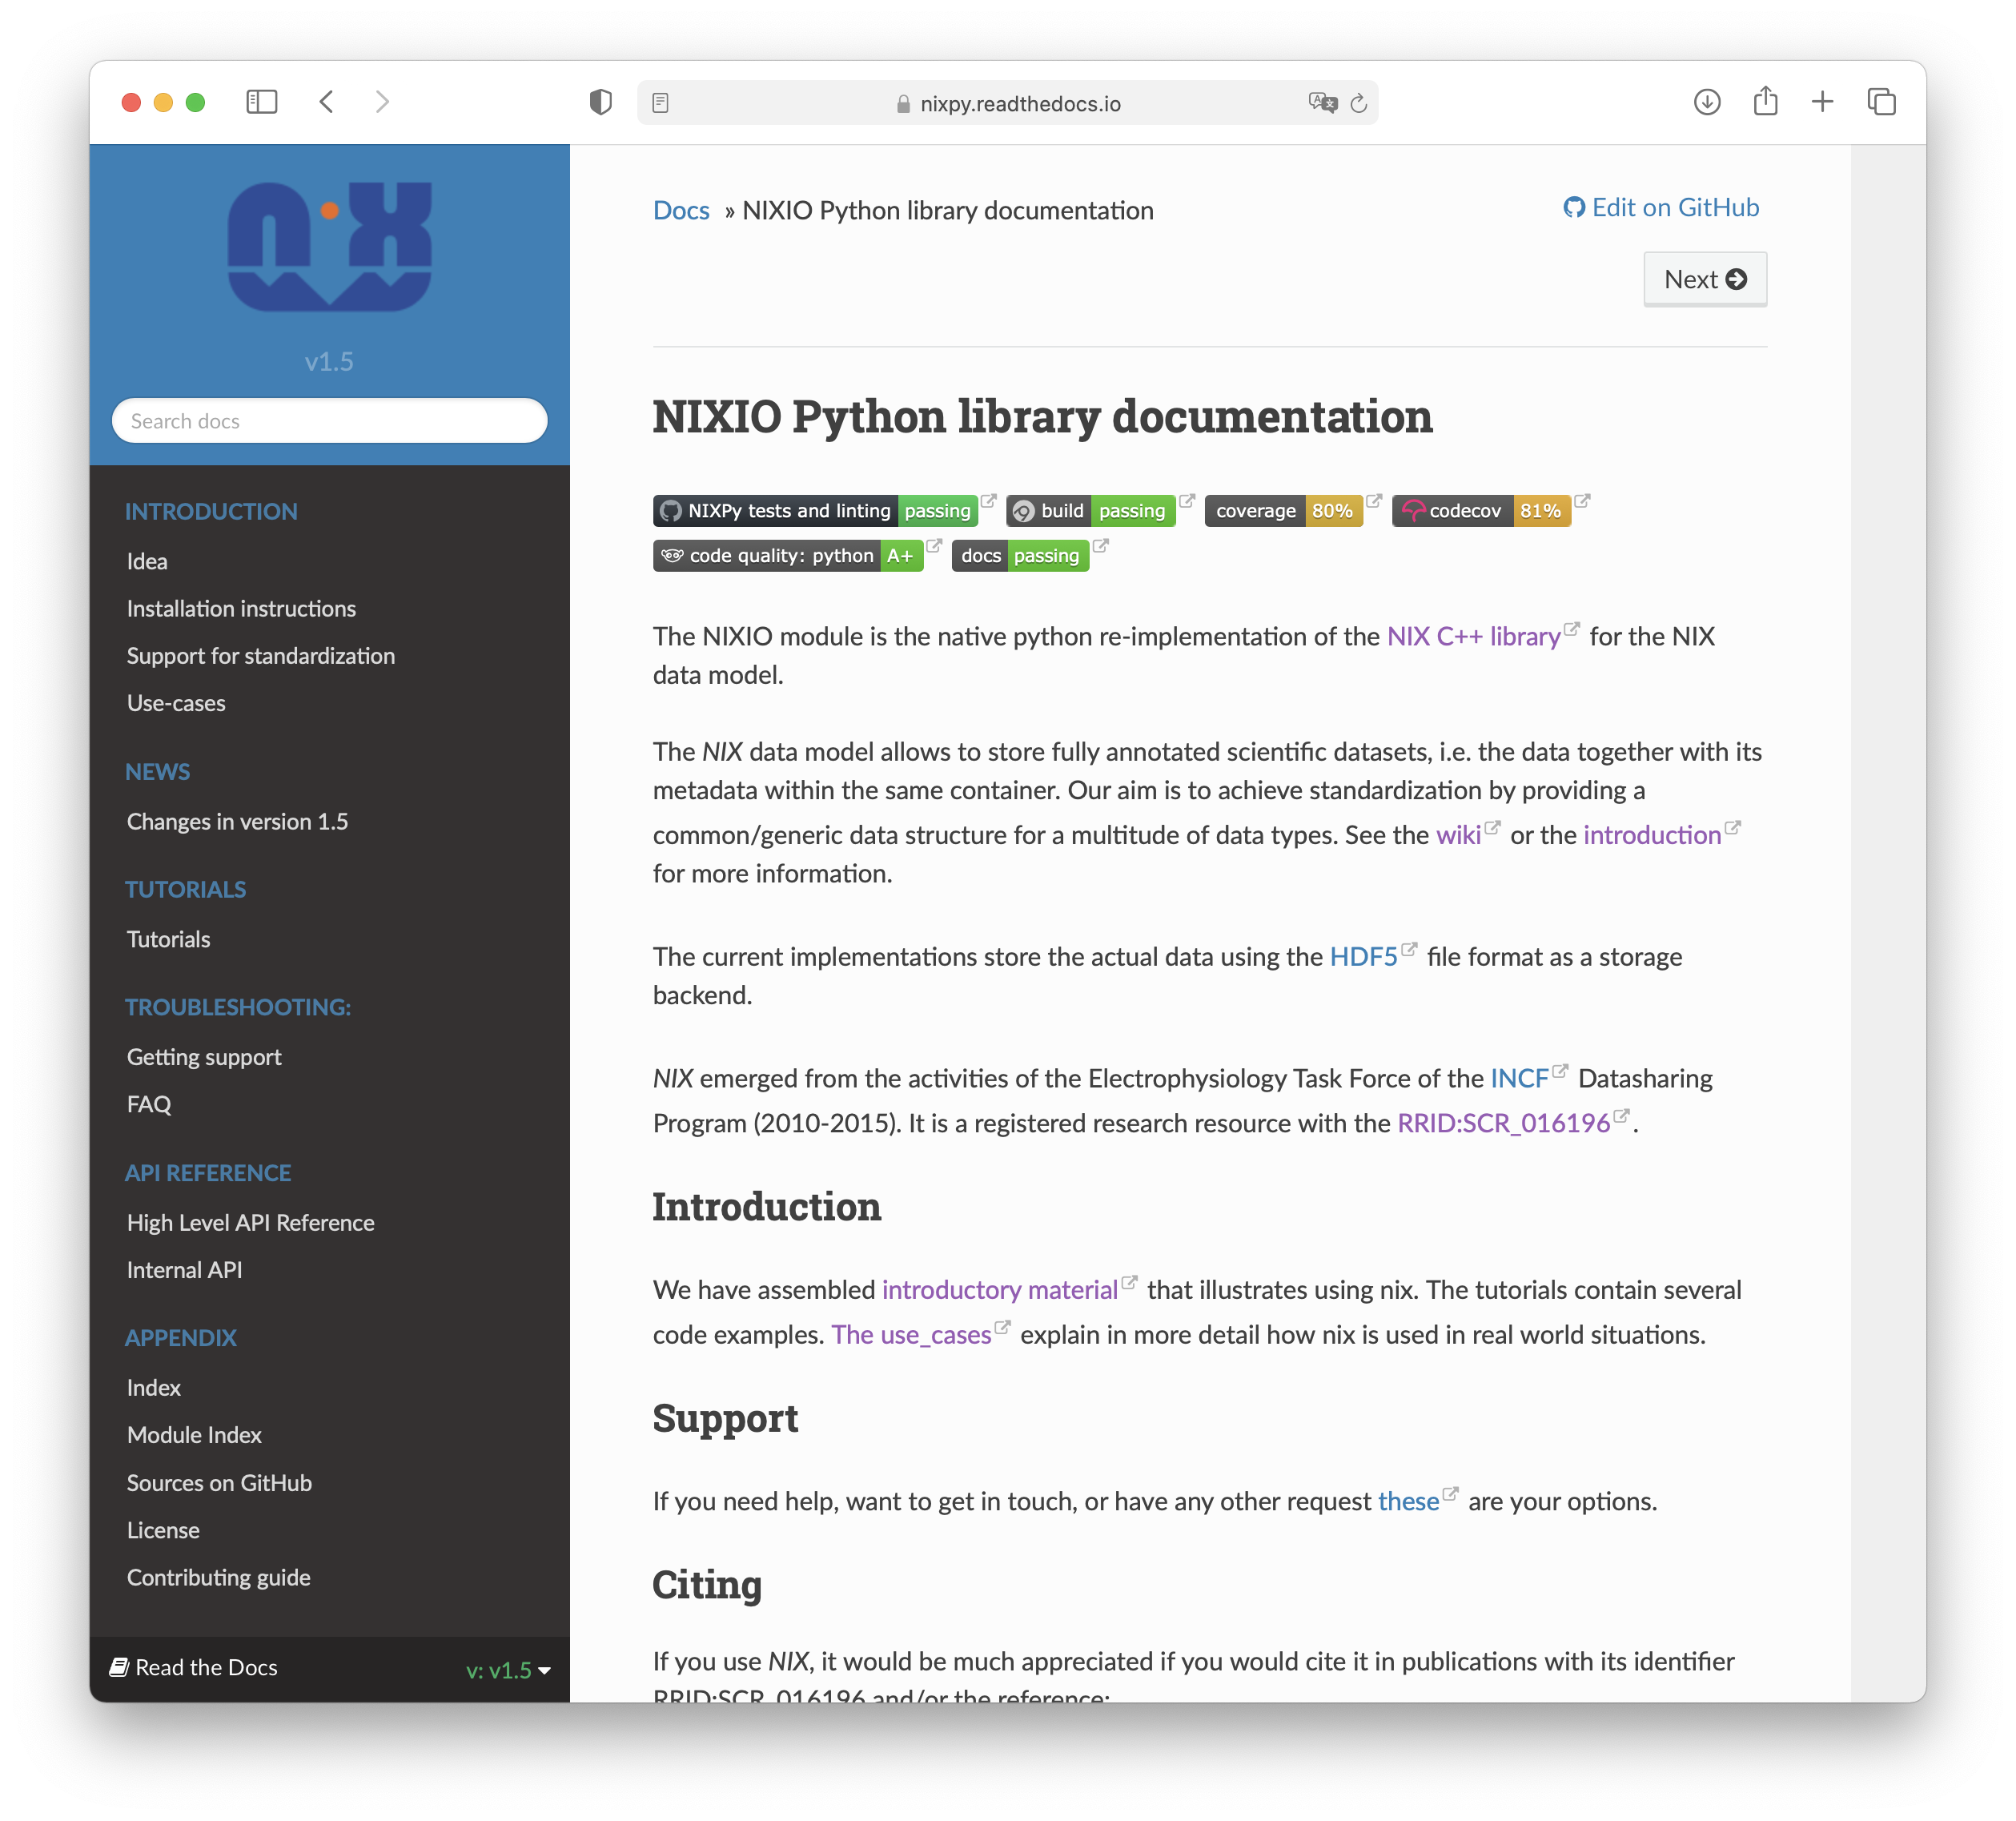
\includegraphics[width=0.7\columnwidth]{resources/rtd_main.png}
    \end{center}
    }\only<2> {
    \begin{center}
        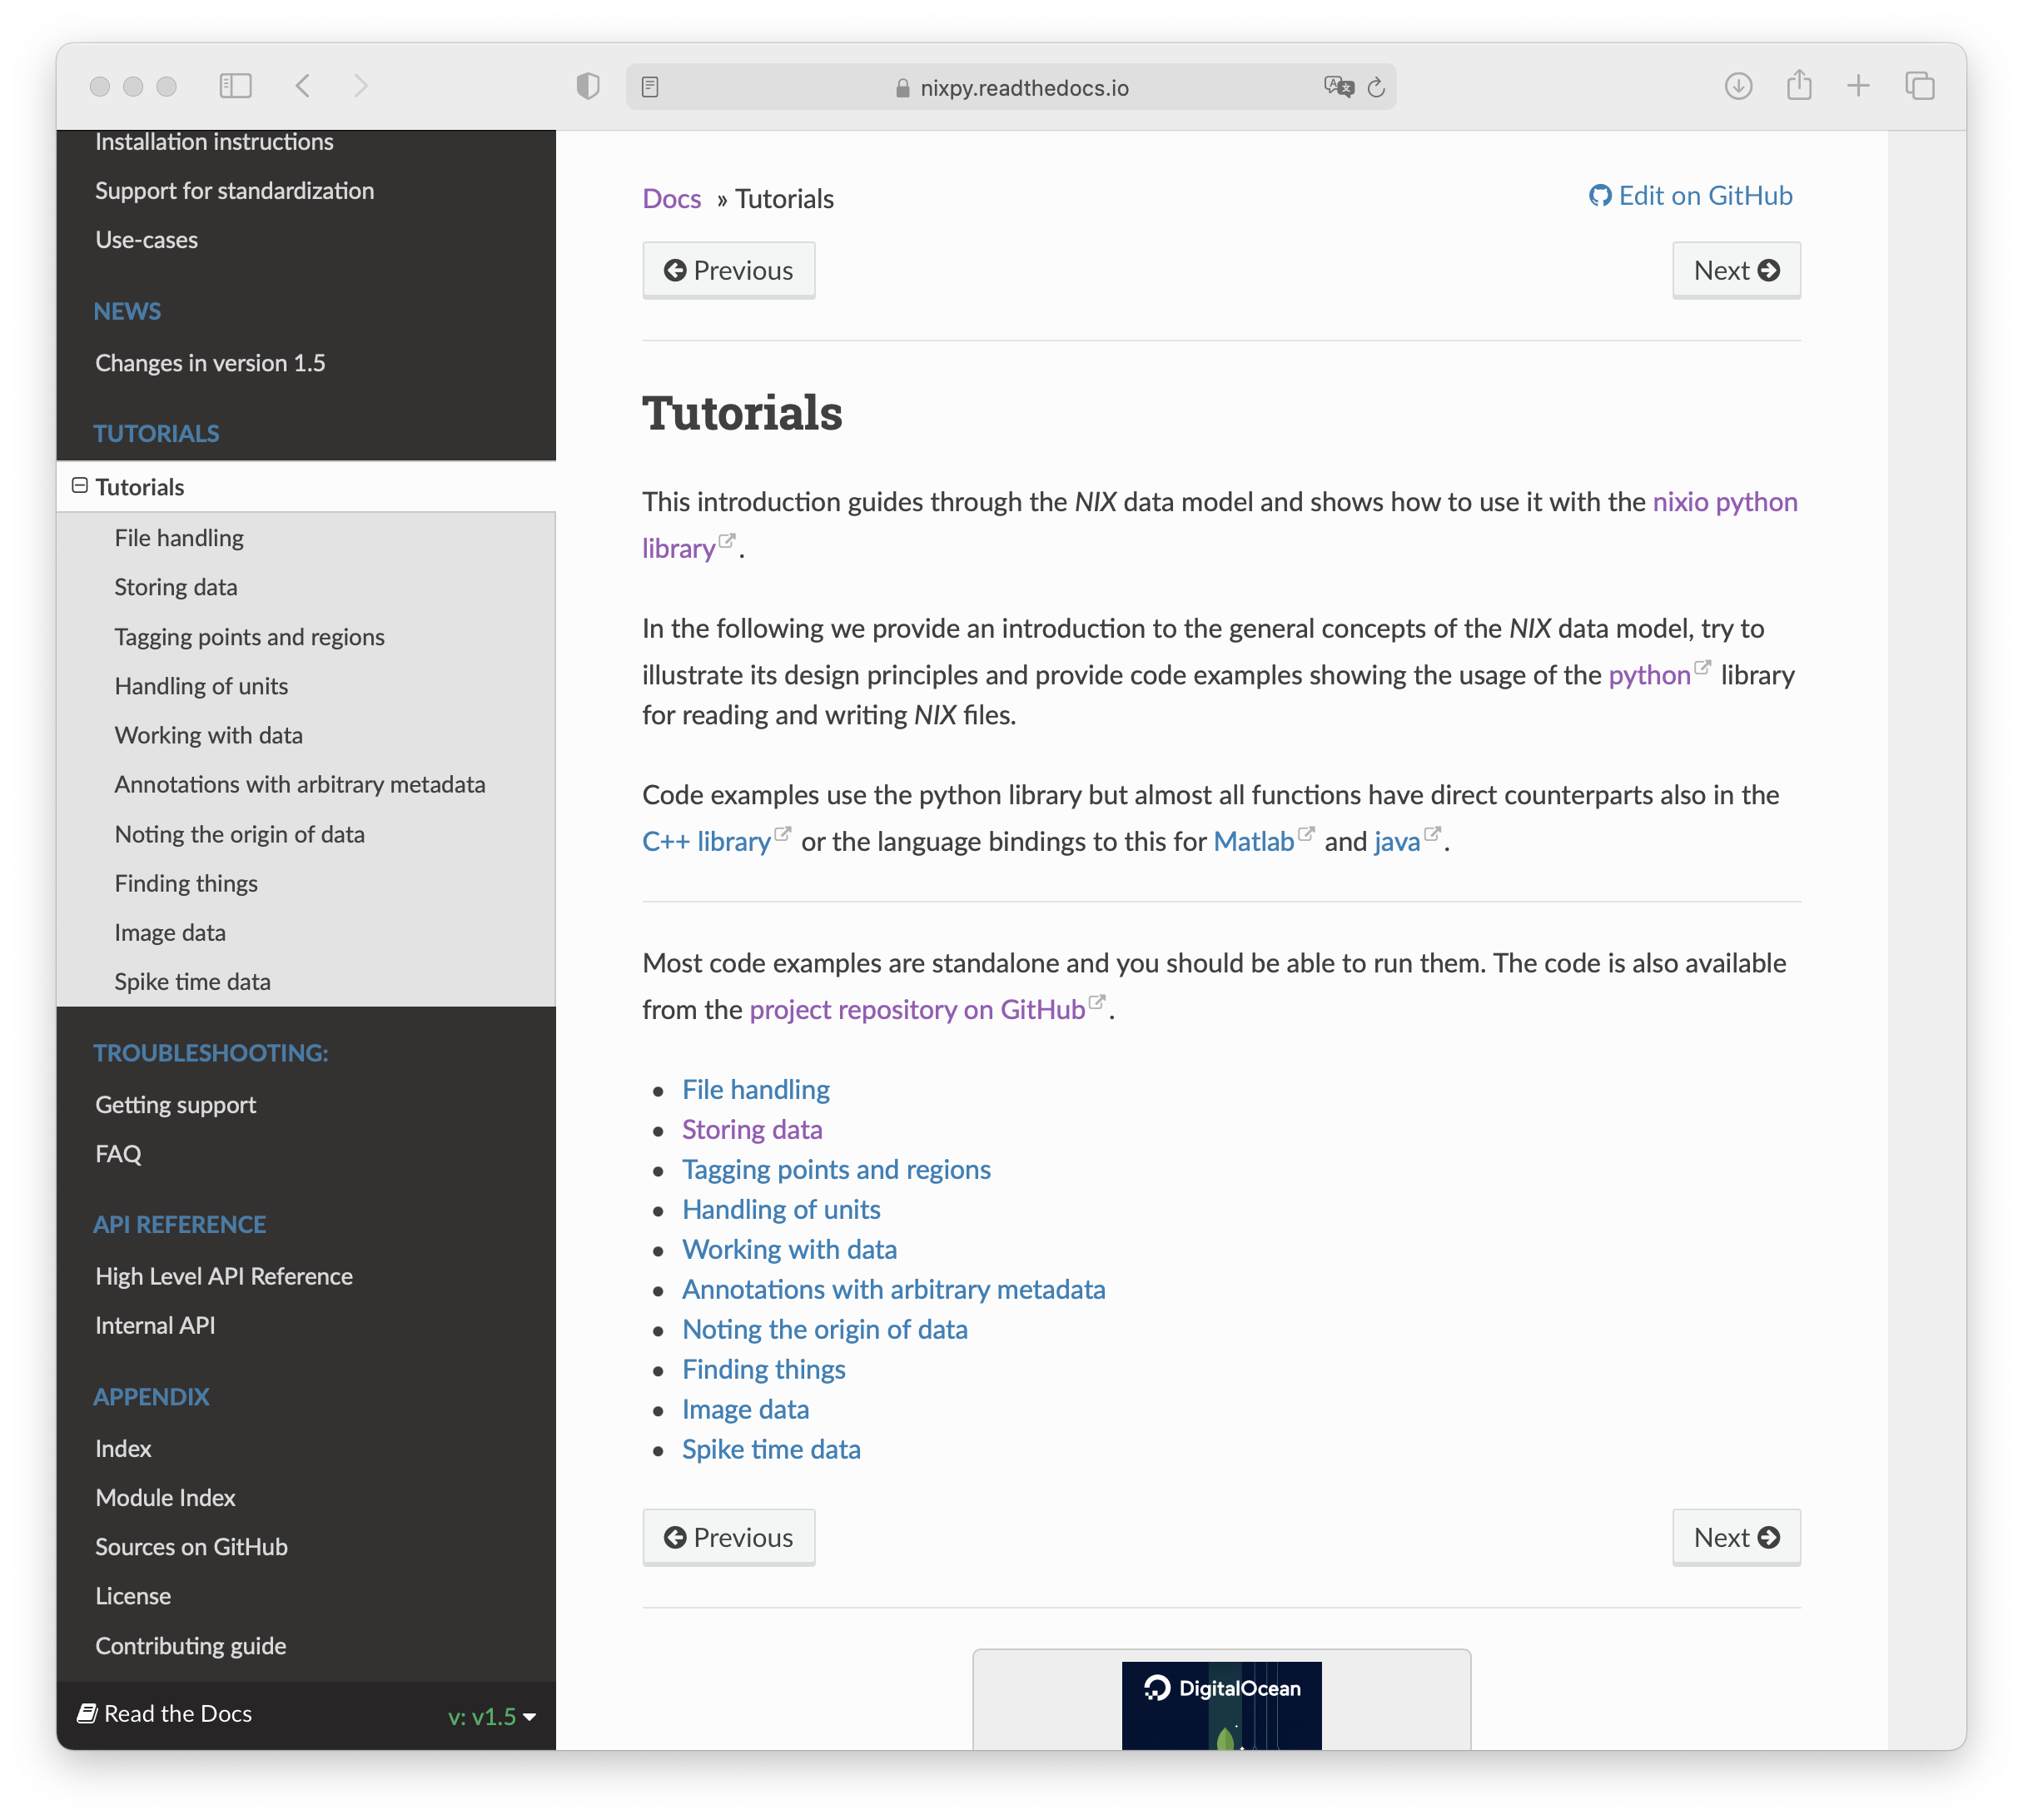
\includegraphics[width=0.7\columnwidth]{resources/rtd_tutorials.png}
    \end{center}
    }
\end{frame}

\end{document}
